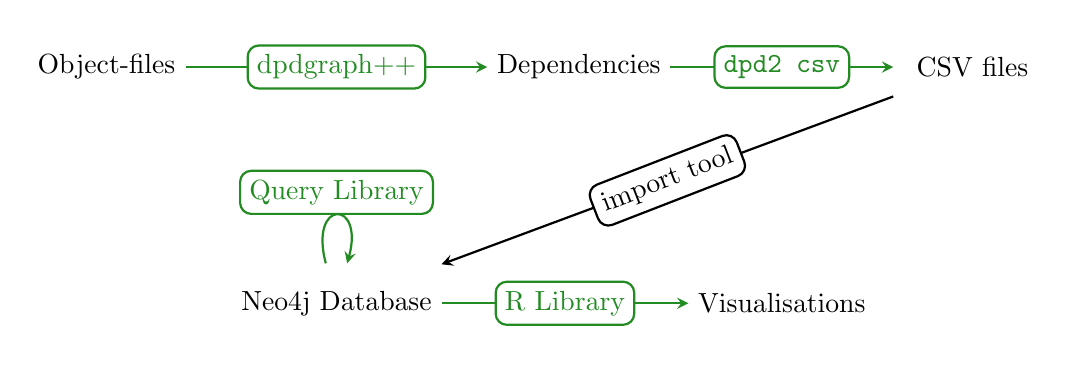
\begin{tikzpicture}[every loop/.style={}]
  \tikzstyle{phase} = [
    rectangle,
    % rounded corners,
    minimum width=2cm,
    minimum height=1cm,
    text centered,
    % draw=black,
  ]

  \tikzstyle{me} = [ thick, ->, >=stealth, color=ForestGreen ]
  \tikzstyle{metoo} = [ rounded corners, draw=ForestGreen, fill=white, text centered, text=ForestGreen ]
  \tikzstyle{notme} = [ thick, ->, >=stealth  ]

  \node (compiled-coq) [phase] {Object-files};
  \node (dpd-file) [phase, xshift=5cm, right of=compiled-coq] {Dependencies};
  \node (csv) [phase, xshift=4cm, right of=dpd-file] {CSV files};

  \draw [me] (compiled-coq) -- node[name=dpdgraph, metoo] {dpdgraph++} (dpd-file);
  \draw [me] (dpd-file) -- node[name=dpd2csv, metoo] {\texttt{dpd2 csv}} (csv);

  \node (neo4j-db) [phase, yshift=-2cm, below of=dpdgraph] {Neo4j Database};
  \node (visual) [phase, yshift=-2cm, below of=dpd2csv] {Visualisations};

  \draw [notme] (csv) -- node[rounded corners, draw=black, rotate=21.2, fill=white] {import tool} (neo4j-db);
  \path [me] (neo4j-db) edge[loop above] node[anchor=south, metoo] {Query Library} (neo4j-db);
  \draw [me] (neo4j-db) -- node[metoo] {R Library} (visual);

\end{tikzpicture}
